
\title{T-61.5130 Machine Learning and Neural Networks}
\author{Karhunen, Luttinen}
\date{Exercise 5, ??.??.2012}

\newcommand{\vect}[1]{{\bf{#1}}}
\newcommand{\svect}[1]{\boldsymbol{#1}}
\newcommand{\matr}[1]{\boldsymbol{#1}}


\begin{document}

\maketitle

\begin{enumerate}
  
\item In the steepest descent method the adjustment
  $\Delta\mathbf{w}(n)$ applied to the parameter vector
  $\mathbf{w}(n)$ is defined by
  $\Delta\mathbf{w}(n)=-\eta\mathbf{g}(n)$, where $\eta$ is the
  learning-rate parameter and
  \begin{equation*}
    \mathbf{g}(n)=\left.\frac{\partial
        \mathcal{E}_{av}(\mathbf{w})}{\partial \mathbf{w}}\right|_{\mathbf{w}=\mathbf{w}(n)}
  \end{equation*}
  is the local gradient vector of cost
  function $\mathcal{E}_{av}(\mathbf{w})$ averaged over the learning
  samples. How could you determine the learning rate parameter $\eta$ so
  that it minimizes the cost function $\mathcal{E}_{av}(\mathbf{w})$ as much as possible?

  \begin{solution}

    Depending on the nature of $\mathcal{E}_{av}(\mathbf{w})$ the above
    problem can be solved iteratively or analytically.

    While many possible line search methods exist,
    optimal $\eta$ can be found for example as follows:

    Take first some suitable guess for $\eta$, say $\eta_0$. Then compute
    $\mathcal{E}_{av}(\mathbf{w}(n)-\eta_0\mathbf{g}(n))$. If this is
    greater than $\mathcal{E}_{av}(\mathbf{w}(n))$, take a new point
    $\eta_1$ from the search line between $\mathbf{w}(n)$ and
    $\mathbf{w}(n)-\eta_0\mathbf{g}(n)$. Otherwise, choose $\eta_1>\eta_0$
    to see if a larger value of $\eta$ yields an even smaller value
    $\mathcal{E}_{av}(\mathbf{w}(n)-\eta_1\mathbf{g}(n))$. Continue this
    procedure until the optimal $\eta$, with a given precision, is reached.

    The simplest way to implement such a iterative search would be to
    divide the search line into equal intervals so that
    \begin{eqnarray*}
      \eta_1&=&\eta_0/2, \mbox{ if
      }\mathcal{E}_{av}(\mathbf{w}(n)-\eta_0\mathbf{g}(n))>\mathcal{E}_{av}(\mathbf{w}(n))\\
      \eta_1&=&2\eta_0, \mbox{otherwise}
    \end{eqnarray*}
    when we have found the interval where the minimum lies, we can divide
    it again into two parts and get a better estimate of $\eta^*$ and continue in a similar manner.

    Dividing the search interval into two equal parts is not optimal with
    respect to the number of iterations needed to find the optimal
    learning rate parameter. A better way is to use Fibonacci numbers (golden intersection) that
    can be used for optimal division of a search interval.
    % 
    % 
    % \vskip -2cm
    \begin{figure}[h]
      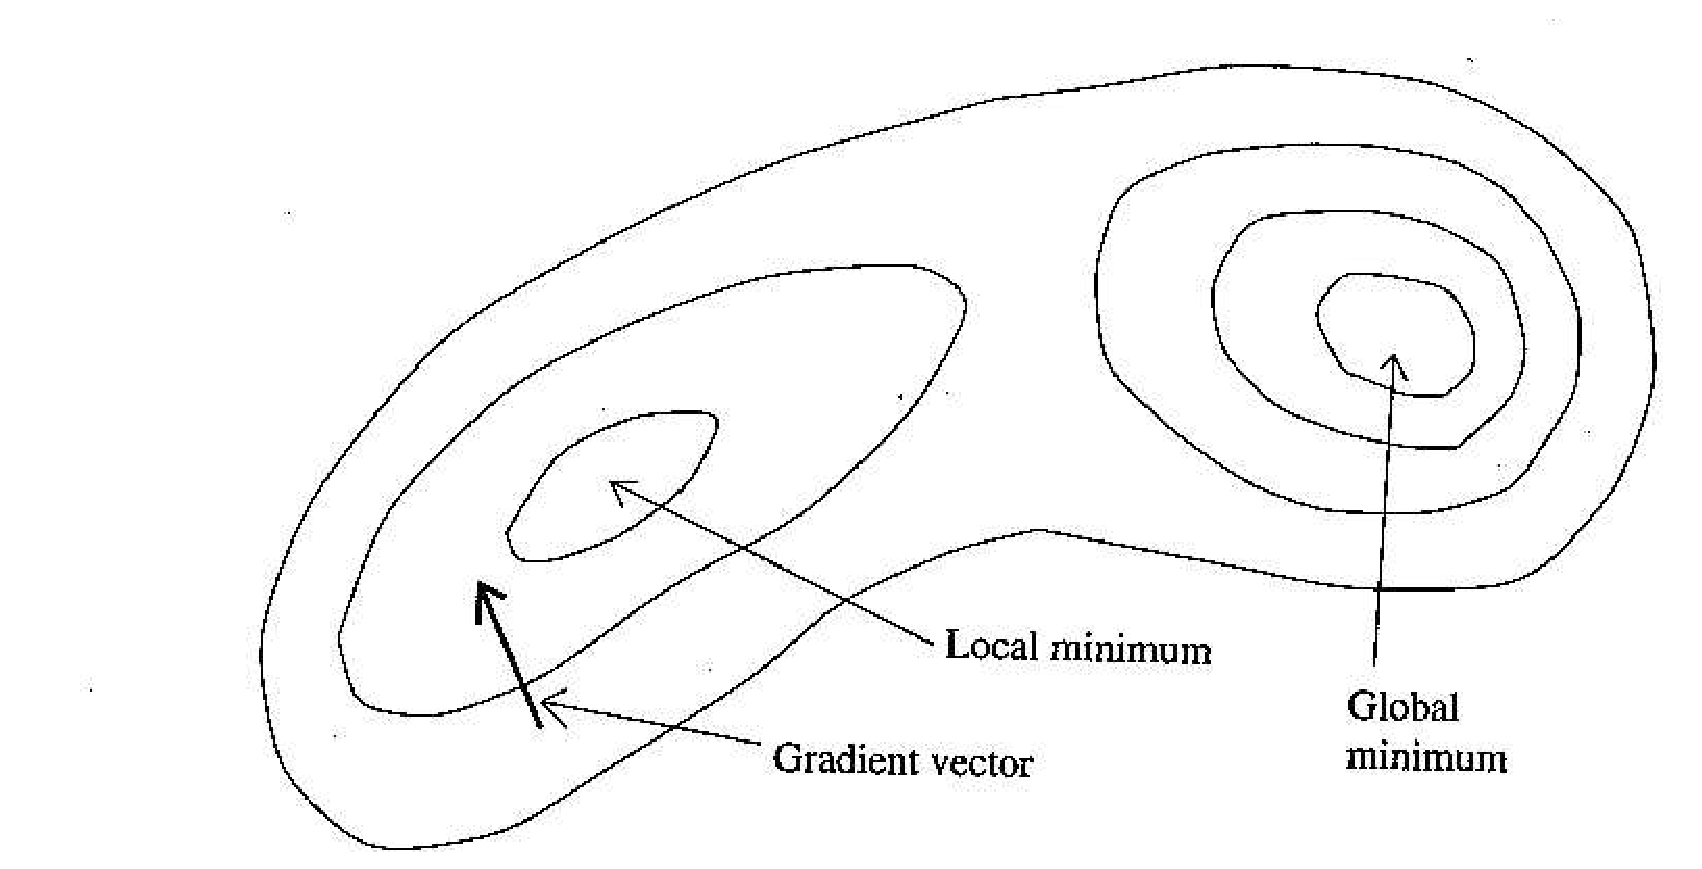
\includegraphics[height=3.5cm]{fig1.eps}
      \caption{Gradient gives the direction of steepest descent at a point. The figure demonstrates
        the fact that the gradient descent method with line search always finds a local minimum, but not necessarily
        the global one.}       
    \end{figure}
    \clearpage

  \end{solution}
  

\item In Ham's and Kostanic's book, the Levenberg-Marquardt algorithm is derived
  in subsection 3.4.4 as an approximation from Newton's optimization algorithm.
  Derive the Levenberg-Marquardt algorithm in another way by linearizing
  the dependence of the errors $e_p$ on the weight vector ${\bf w}$ using
  Taylor series expansion.

  \begin{solution}

    Optimization algorithms:

    Steepest descent: Move iteratively to the direction of the negative gradient.
    \[
    \vect{w}(n+1) = \vect{w}(n) - \eta \vect{g}(n)
    \]

    Newton's method: Use a quadratic approximation of the cost function by
    computing the Hessian matrix
    \[
    \vect{w}(n+1) = \vect{w}(n) - \matr{H}^{-1}(n) \vect{g}(n)
    \]

    Gauss-Newton: Simplified version of Newton's method (no Hessian required)

    \[
    \vect{w}(n+1) = \vect{w}(n) - (\matr{J}(n)^T\matr{J}(n))^{-1} \matr{J}(n)^T \vect{e}(n)
    \]


    The Gauss-Newton method is applicable to a cost function that is
    expressed as the sum of error squares. Let
    \[
    \mathcal{E}(\vect{w})=\frac{1}{2}\sum_{i=1}^{n} e^2(i)
    \]
    where the scaling factor $1/2$ is included to simplify further
    computations. All the error terms in this formula are calculated on
    the basis of a weight vector $\vect{w}$ that is fixed over the the entire
    observation interval $1\leq i\leq n$.

    The error signal $e(i)$ is a function of the adjustable weight vector
    $\vect{w}$. Given an operating point $\vect{w}(n)$, we linearize the dependence of $e(i)$
    on $\vect{w}$ by writing
    \[
    \tilde{e}(i,\vect{w})=e(i) + \left[ \frac{\partial e(i)}{\partial \vect{w}}
    \right]_{\vect{w}=\vect{w}(n)}^{T} \left(
      \vect{w}-\vect{w}(n)\right), \hspace{4mm} i=1,2,...,n
    \]
    Equivalently, in matrix notation we can write
    \[
    \tilde{\vect{e}}(n,\vect{w})=\vect{e}(n)+\matr{J}(n)(\vect{w}-\vect{w}(n))
    \]
    where $\vect{e}(n)$ is the error vector
    \[
    \vect{e}(n)=\left[ e(1), e(2), ... , e(n) \right]^T
    \]
    and $\matr{J}(n)$ is the $n$-by-$m$ Jacobian (matrix of all
    first-order partial derivatives of a vector-valued function).
    \[
    \matr{J}(n)=
    \left[ \begin{array}{cccc}
        \frac{\partial e(1)}{\partial w_1} & \frac{\partial e(1)}{\partial w_2} & \cdots & \frac{\partial e(1)}{\partial w_m} \\
        \frac{\partial e(2)}{\partial w_1} & \frac{\partial e(2)}{\partial w_2} & \cdots & \frac{\partial e(2)}{\partial w_m} \\
        \vdots & \vdots & \ddots &  \vdots \\
        \frac{\partial e(n)}{\partial w_1} & \frac{\partial e(n)}{\partial w_2} & \cdots & \frac{\partial e(n)}{\partial w_m} 
      \end{array} \right]_{\vect{w}=\vect{w}(n)}
    \]
    The Jacobian matrix $\matr{J}(n)$ is the transpose of the $m$-by-$n$ gradient matrix $\nabla \vect{e}(n)$, where
    \[
    \nabla \vect{e}(n) = \left[ \nabla e(1),\nabla e(2), ... ,\nabla e(n) \right]
    \]
    The updated weight vector $\vect{w}(n+1)$ is then defined by
    \[
    \vect{w}(n+1)=\arg \min_{\vect{w}} \{ \frac{1}{2} \| \tilde{\vect{e}}(n,\vect{w})\|^2\rbrace
    \]
    Using the approximation for the Euclidian squared norm of
    $\vect{e}(n,\vect{w})$, we get
    \[
    \frac{1}{2} \| \tilde{\vect{e}}(n,\vect{w}) \|^2 = \frac{1}{2} \|\vect{e}(n)\|^2 + \vect{e}^T(n)\matr{J}(n)(\vect{w}-\vect{w}(n)) + \frac{1}{2}(\vect{w}-\vect{w}(n))^T\matr{J}^T(n)\matr{J}(n)(\vect{w}-\vect{w}(n))
    \]
    Hence, differentiating this expression with respect to $\vect{w}$ and setting the result equal to zero, we obtain
    \[
    \matr{J}^T(n)\vect{e}(n) + \matr{J}^T(n)\matr{J}(n)(\vect{w}-\vect{w}(n))=\vect{0}
    \]
    and solving this for $\vect{w}$ results in
    \[
    \vect{w}(n+1) = \vect{w}(n) - \left(\matr{J}^T(n)\matr{J}(n)\right)^{-1}\matr{J}^T(n)\vect{e}(n)
    \]

    However, to ensure that the matrix $\matr{J}^T(n)\matr{J}(n)$ is
    nonsingular (invertible) we can add a small increment $\sigma$ to the
    diagonal of the matrix resulting in the update rule
    \[
    \vect{w}(n+1) = \vect{w}(n) - \left(\matr{J}^T(n)\matr{J}(n) + \sigma
      \matr{I} \right)^{-1}\matr{J}^T(n)\vect{e}(n)
    \]
    which is the Levenberg-Marquardt learning rule.
  \end{solution}


\item In extreme learning machine, the optimal weights are computed using the
  pseudoinverse ${\bf H}^+$ of the hidden layer output matrix ${\bf H}$. Consider
  an $N \times M$ matrix ${\bf X}$, which is generally rectangular with $N \neq M$.
  The singular value decomposition (SVD) of ${\bf X}$ is a generalization of the
  eigendecomposition, defined for square matrices only, to rectangular matrices.
  Similarly, the pseudoinverse ${\bf X}^+$ of ${\bf X}$ is a generalization of the
  standard inverse matrix defined for square non-singular matrices only to
  rectangular matrices. Discuss the definitions, computation, and interrelationships
  of the SVD and pseudoinverse of ${\bf X}$.

  \begin{solution}

    These important concepts may already be familiar to you from courses of mathematics,
    but it is useful to recall them here.

    Consider first the singular value decomposition of ${\bf X}$. It is defined by
    % 
    \begin{equation}
      {\bf X} = {\bf USV}^T
      \label{eq:SVD}
    \end{equation}
    % 
    where ${\bf U}$ = $[{\bf u}_1,{\bf u}_2,\ldots,{\bf u}_N]$ and ${\bf V}$ =
    $[{\bf v}_1,{\bf v}_2,\ldots,{\bf v}_M]$ are $N \times N$ and $M \times M$
    orthogonal matrices, respectively. Thus ${\bf U}^T{\bf U}$ = ${\bf I}_{N \times N}$,
    where ${\bf I}_{N \times N}$ is $N \times N$ unit matrix, and similarly
    ${\bf V}^T{\bf V}$ = ${\bf I}_{M \times M}$ is $M \times M$ unit matrix. This means
    that the column vectors ${\bf u}_i$ of ${\bf U}$, called the left singular vectors
    of ${\bf X}$, are mutually orthonormal. Similarly the right singular vectors
    ${\bf v}_i$ of ${\bf X}$ that are the column vectors of ${\bf V}$ are mutually
    orthonormal.

    The matrix ${\bf S}$ in (\ref{eq:SVD}) is an $N \times M$ non-negative pseudodiagonal
    matrix defined by 
    % 
    \begin{equation}
      {\bf S} = \left[ \begin{array}{cc}
          {\bf D} & {\bf 0} \\
          {\bf 0} & {\bf 0} \end{array} \right]
      \label{eq:Smatrix}
    \end{equation}
    % 
    There 
    % 
    \begin{equation}
      {\bf D} = \mbox{diag}(\sigma_1,\sigma_2,\ldots,\sigma_L)
      \label{eq:Dmatrix}
    \end{equation}
    % 
    where the $L$ positive numbers 
    % 
    \begin{equation}
      \sigma_1 \geq \sigma_2 \geq \ldots \geq \sigma_L > 0
      \label{eq:singvalues}
    \end{equation}
    % 
    together with $\sigma_{L+1} = \ldots = \sigma_M = 0$ are called the singular values
    of matrix ${\bf X}$. Only the nonzero singular values (\ref{eq:singvalues}) are of
    any real interest. All the elements of the zero matrices ${\bf 0}$ in (\ref{eq:Smatrix})
    are zero. They have compatible dimensions so that they complement the $L \times L$
    diagonal matrix ${\bf D}$ to the $N \times M$ pseudodiagonal matrix ${\bf S}$.

    The right hand side of (\ref{eq:SVD}) can be expanded to
    % 
    \begin{equation}
      {\bf X} = \sum_{i=1}^L \sigma_i {\bf u}_i {\bf v}_i^T
      \label{eq:SVDexp}
    \end{equation}
    % 
    The outer products ${\bf u}_i {\bf v}_i^T$ form a set of unit-rank matrices, each
    of which is scaled by the corresponding $i$:th singular value $\sigma_i$ of the
    matrix ${\bf X}$. Thus the rank of the matrix ${\bf X}$ equals the number $L$ of
    its positive singular values.

    Using the orthonormality of the singular vectors, it is easy to see from
    (\ref{eq:SVDexp}) that 
    % 
    \begin{equation}
      {\bf Xv}_i = \left\{ \begin{array}{cl}
          \sigma_i {\bf u}_i, & i=1,2,\ldots,L \\
          {\bf 0}, & i=L+1,\ldots,M 
        \end{array} \right.
      \label{eq:Xvi}
    \end{equation}
    % 
    and 
    % 
    \begin{equation}
      {\bf X}^T{\bf u}_i = \left\{ \begin{array}{cl}
          \sigma_i {\bf v}_i, & i=1,2,\ldots,L \\
          {\bf 0}, & i=L+1,\ldots,N 
        \end{array} \right.
      \label{eq:XTui}
    \end{equation}
    % 
    Postmultiplying the both sides of (\ref{eq:Xvi}) by ${\bf X}^T$ and then utilizing
    (\ref{eq:XTui}), we get easily
    % 
    \begin{equation}
      {\bf X}^T{\bf Xv}_i = \left\{ \begin{array}{cl}
          \sigma_i^2 {\bf v}_i, & i=1,2,\ldots,L \\
          {\bf 0}, & i=L+1,\ldots,M 
        \end{array} \right.
      \label{eq:XTXvi}
    \end{equation}
    % 
    This result shows that the right singular vectors ${\bf v}_i$ of ${\bf X}$ are the
    eigenvectors of the matrix ${\bf X}^T{\bf X}$, and the $M$ singular values of 
    ${\bf X}$ are the non-negative square roots of the eigenvalues of the matrix
    ${\bf X}^T{\bf X}$.

    Similarly, it is easy to see that
    % 
    \begin{equation}
      {\bf XX}^T{\bf u}_i = \left\{ \begin{array}{cl}
          \sigma_i^2 {\bf u}_i, & i=1,2,\ldots,L \\
          {\bf 0}, & i=L+1,\ldots,N 
        \end{array} \right.
      \label{eq:XXTui}
    \end{equation}
    % 
    Thus the left singular vectors ${\bf u}_i$ of ${\bf X}$ are the eigenvectors of the
    matrix ${\bf XX}^T$. Equation (\ref{eq:XXTui}) also shows that the $N$ eigenvalues of 
    ${\bf XX}^T$ are the squares of the singular values of ${\bf X}^T$.

    In practice, one can first computer either the left or right singular vectors
    as eigenvectors of the smaller dimensional of the $N \times N$ and $M \times M$
    square matrices ${\bf XX}^T$ and ${\bf X}^T{\bf X}$, respectively. The other
    set of singular vectors can then be calculated easily from the linear transformations
    (\ref{eq:Xvi}) or (\ref{eq:XTui}) without needing to compute the eigendecomposition
    of the larger dimensional matrix.

    Note also that for symmetric square matrices ${\bf X}^T = {\bf X}$, the left and
    right singular vectors become the same, ${\bf U} = {\bf V}$, and the SVD of the matrix
    ${\bf X}$ reduces to its eigendecomposition. Therefore for example principal component
    analysis, which is defined in terms of the eigendecomposition data covariance matrix,
    can be defined in terms of the SVD of the data covariance matrix as well.

    Consider then the pseudoinverse ${\bf X}^+$ of the generally rectangular $N \times M$
    matrix ${\bf X}$. It is defined in terms of the singular value decomposition
    (\ref{eq:SVD}) of ${\bf X}$ as the $M \times N$ matrix
    % 
    \begin{equation}
      {\bf X}^+ = {\bf VS}^+{\bf U}^T
      \label{eq:pinv}
    \end{equation}
    % 
    where ${\bf S}^+$ is the $M \times N$ matrix
    % 
    \begin{equation}
      {\bf S}^+ = \left[ \begin{array}{cc}
          {\bf D}^{-1} & {\bf 0} \\
          {\bf 0} & {\bf 0} \end{array} \right]
      \label{eq:Splus}
    \end{equation}
    % 
    There ${\bf D}^{-1}$ is a diagonal $L \times L$ matrix whose diagonal elements are
    the reciprocals of the $L$ nonzero singular values of ${\bf X}$, that is
    % 
    \begin{equation}
      {\bf D}^{-1} = \mbox{diag}(\sigma_1^{-1},\sigma_2^{-1},\ldots,\sigma_L^{-1})
      \label{eq:Dinv}
    \end{equation}
    % 
    where $L$ is the rank of ${\bf X}$.

    Expanding the right hand side of (\ref{eq:pinv}), we can express the pseudoinverse
    ${\bf X}^+$ as
    % 
    \begin{equation}
      {\bf X}^+ = \sum_{i=1}^L \sigma_i^{-1} {\bf v}_i {\bf u}_i^T
      \label{eq:pinvexp}
    \end{equation}
    % 
    where $\sigma_i$ is the $i$:th singular value of ${\bf X}$, and ${\bf u}_i$ and
    ${\bf v}_i$ are the associated left and right singular vectors, respectively.

    The pseudoinverse ${\bf X}^+$ has the following properties:
    % 
    \begin{enumerate}
    \item  The dimensions of ${\bf X}^+$ are the reversed dimensions of ${\bf X}$.
      Hence the product ${\bf XX}^+$ or ${\bf X}^+{\bf X}$ is a square matrix.
    \item The nonzero singular values of ${\bf X}^+$ are the reciprocals of the
      corresponding singular values of ${\bf X}$; their number is the rank of ${\bf X}$.
    \item The left singular vector of ${\bf X}^+$ are the right singular vectors of
      ${\bf X}$, and vice versa.
    \end{enumerate}
    % 
    The last two properties are easily verified by comparing the expansion
    (\ref{eq:pinvexp}) with (\ref{eq:SVDexp}).

    Depending on the rank of ${\bf X}$, the pseudoinverse ${\bf X}^+$ has the following
    special forms: 
    % 
    \begin{enumerate}
    \item If the rank of ${\bf X}$ is $L=M$, then
      % 
      \begin{equation}
        {\bf X}^+ = ({\bf X}^T{\bf X})^{-1}{\bf X}^T, \hspace{1cm} L=M
        \label{eq:LM}
      \end{equation}
      % 
      Hence the product ${\bf X}^+{\bf X}$ is $M \times M$ unit matrix ${\bf I}_{M \times M}$.
      % 
    \item If the rank of ${\bf X}$ is $L=N$, then
      % 
      \begin{equation}
        {\bf X}^+ = {\bf X}^T({\bf XX}^T)^{-1}, \hspace{1cm} L=N
        \label{eq:LN}
      \end{equation}
      % 
      Hence the product ${\bf XX}^+$ is $N \times N$ unit matrix ${\bf I}_{N \times N}$.
      % 
    \item If ${\bf X}$ is a square matrix (that is, $M=N$), and its rank $L=M=N$, then
      the pseudoinverse ${\bf X}^+$ is the inverse of ${\bf X}$:
      % 
      \begin{equation}
        {\bf X}^+ = {\bf X}^{-1}, \hspace{1cm} L=N=M
        \label{eq:LNM}
      \end{equation}
      % 
    \end{enumerate}
    % 
    One can prove these results fairly easily by inserting the expansion (\ref{eq:SVDexp})
    into (\ref{eq:LM}) and (\ref{eq:LN}), noticing that the matrices to be inverted there
    have full rank and hence their inverses exist, and then verifying that the result is
    the expansion (\ref{eq:pinvexp}) of the pseudoinverse ${\bf X}^+$.

    The pseudoinverse of a matrix is closely related to solution of linear equations in 
    various cases. Consider first the standard matrix-vector formulation 
    % 
    \begin{equation}
      {\bf X}{\bf y} = {\bf a}
      \label{eq:Xya}
    \end{equation}
    % 
    of linear equations, where ${\bf X}$ is known $N \times M$ coefficient matrix,
    the vector ${\bf y}$ contains the $M$ unknowns to be solved, and ${\bf a}$ is
    known $N$-dimensional target vector. The most desirable minimum norm solution is in
    all cases given by
    % 
    \begin{equation}
      {\bf y} = {\bf X}^+{\bf a}
      \label{eq:y}
    \end{equation}
    % 
    where the pseudoinverse ${\bf X}^+$ is defined in different cases from the equations
    (\ref{eq:LM}), (\ref{eq:LN}), and (\ref{eq:LNM}). 

    First, if $N > M$, there are more equations ($N$) than unknowns ($M$) in the set
    of linear equations (\ref{eq:Xya}), and there is usually no solution. The best
    approximative solution is usually constructed by minimizing the squared error
    $\parallel {\bf e} \parallel^2$ in the equation
    % 
    \begin{equation}
      {\bf X}{\bf y} = {\bf a} + {\bf e}
      \label{eq:lseq}
    \end{equation}
    % 
    which leads to the least-squares solution (\ref{eq:LM}), (\ref{eq:y}). Second,
    if $N <M$, there are less equations than unknowns in (\ref{eq:Xya}), and there
    usually exists infinitely many solutions. The pseudoinverse (\ref{eq:LN}) gives
    again the minimum norm solution. Finally, the inverse matrix (\ref{eq:LNM})
    provides the unique solution in the case where there are as many equations as
    unknowns ($M=N$) in (\ref{eq:Xya}), and the matrix ${\bf X}$ has full rank
    $L = M = N$.

    These results generalize easily for the matrix-matrix equation
    % 
    \begin{equation}
      {\bf XY} = {\bf A}
      \label{eq:XYA}
    \end{equation}
    % 
    where ${\bf Y}$ is now $M \times K$ matrix and ${\bf A}$ $N \times K$ matrix. The
    solution is again given by 
    % 
    \begin{equation}
      {\bf Y} = {\bf X}^+{\bf A}
      \label{eq:Y}
    \end{equation}
    % 
    where the pseudoinverse ${\bf X}^+$ of ${\bf X}$ is defined quite similarly as above in 
    different cases from the equations (\ref{eq:LM}), (\ref{eq:LN}), and (\ref{eq:LNM}).
    Note that the extra dimension $K$ does not have any effect here.

    Finally, we can apply these results to the extreme learning machine, where the solution
    of the equations ${\bf HB} = {\bf T}$ corresponding to (\ref{eq:XYA}) is
    % 
    \begin{equation}
      {\bf B} = {\bf H}^+{\bf T}
      \label{eq:B}
    \end{equation}
    % 
    Note that the case $N < M$ is not meaningful in practice, because then there are
    more neurons ($M$) in the hidden layer than known input-output pairs ($N$). Perfect
    match can be achieved already if $M = N$.




  \end{solution}
  

\item (Ham \& Kostanic 3.8, Matlab demo) Write a computer program that uses the MLP
  network trained by backpropagation to perform image compression. To
  generate the input/target vectors $\vect{x}$, divide the image into
  8-by-8 pixel blocks and arrange the elements of each block into a
  64-dimensional vector. Experiment with different numbers of neurons
  in the hidden layer.

  \begin{solution}

  \end{solution}
  
\end{enumerate}
\end{document}             % End of document.

%%% Local Variables: 
%%% mode: latex
%%% TeX-master: "ex05_solutions"
%%% End: 
